\documentclass[12pt,a4paper]{article}

% ============================================================
% Package imports
% ============================================================
\usepackage[margin=2.5cm]{geometry}
\usepackage{amsmath}
\usepackage{amssymb}
\usepackage{graphicx}
\usepackage[colorlinks=true,linkcolor=blue,citecolor=blue,urlcolor=blue]{hyperref}
\usepackage[ruled,vlined,linesnumbered]{algorithm2e}
\usepackage{listings}
\usepackage{booktabs}
\usepackage[numbers,sort&compress]{natbib}
\usepackage{fancyhdr}
\usepackage{caption}
\usepackage{subcaption}
\usepackage[dvipsnames]{xcolor}
\usepackage{tikz}
\usetikzlibrary{shapes.geometric, arrows.meta, positioning, fit, backgrounds}
\usepackage{microtype}
\usepackage{setspace}
\usepackage{titlesec}

% ============================================================
% Listings configuration (code blocks)
% ============================================================
\definecolor{codebg}{RGB}{248,248,248}
\definecolor{codecomment}{RGB}{130,130,130}
\definecolor{codekeyword}{RGB}{0,102,204}
\definecolor{codestring}{RGB}{163,21,21}

\lstdefinestyle{rust}{
  language        = {[rust]C},
  backgroundcolor = \color{codebg},
  commentstyle    = \color{codecomment}\itshape,
  keywordstyle    = \color{codekeyword}\bfseries,
  stringstyle     = \color{codestring},
  basicstyle      = \ttfamily\footnotesize,
  breaklines      = true,
  frame           = single,
  framerule       = 0.4pt,
  rulecolor       = \color{gray!40},
  numbers         = left,
  numberstyle     = \tiny\color{gray},
  stepnumber      = 1,
  tabsize         = 4,
  captionpos      = b,
  morekeywords    = {pub, fn, let, mut, struct, enum, impl, use, mod, trait,
                     Self, String, u8, u16, u32, u64, i32, i64, f32, f64,
                     bool, usize, Vec, HashMap, Option, Result, Some, None,
                     Ok, Err, Box, Arc, Rc, iter, collect, unwrap}
}

\lstdefinestyle{bash}{
  language        = bash,
  backgroundcolor = \color{codebg},
  commentstyle    = \color{codecomment}\itshape,
  keywordstyle    = \color{codekeyword},
  basicstyle      = \ttfamily\footnotesize,
  breaklines      = true,
  frame           = single,
  framerule       = 0.4pt,
  rulecolor       = \color{gray!40},
  captionpos      = b
}

\lstset{style=rust}

% ============================================================
% Header / footer
% ============================================================
\pagestyle{fancy}
\fancyhf{}
\fancyhead[L]{\small\textit{kmerdet: K-mer-Based Variant Detection for Liquid Biopsy ctDNA Monitoring}}
\fancyhead[R]{\small\thepage}
\fancyfoot[C]{}
\renewcommand{\headrulewidth}{0.4pt}

% ============================================================
% Section formatting
% ============================================================
\titleformat{\section}
  {\large\bfseries}{\thesection}{1em}{}
\titleformat{\subsection}
  {\normalsize\bfseries}{\thesubsection}{1em}{}
\titleformat{\subsubsection}
  {\normalsize\itshape}{\thesubsubsection}{1em}{}

% ============================================================
% Custom commands
% ============================================================
\newcommand{\kmerdet}{\textsc{kmerdet}}
\newcommand{\km}{\textit{km}}
\newcommand{\kmtools}{\textit{kmtools}}
\newcommand{\kam}{\textit{kam}}
\newcommand{\jf}{Jellyfish}
\newcommand{\ctDNA}{ctDNA}
\newcommand{\rVAF}{rVAF}
\newcommand{\kmer}{$k$-mer}
\newcommand{\kmers}{$k$-mers}
\newcommand{\kval}{$k$}
\newcommand{\todo}[1]{\textbf{\color{red}[TODO: #1]}}

% ============================================================
% Document
% ============================================================
\begin{document}

% ----- Title page -------------------------------------------
\begin{titlepage}
  \centering
  \vspace*{3cm}

  {\Huge\bfseries kmerdet\par}
  \vspace{0.5cm}
  {\Large A High-Performance K-mer-Based Variant Detection Framework\\
   for Liquid Biopsy ctDNA Monitoring\par}

  \vspace{2cm}

  
\begin{tikzpicture}
    \draw[thick, gray!50] (0,0) rectangle (12,0.15);
  \end{tikzpicture}

  \vspace{2cm}

  {\large
    \textbf{Abstract}\par
  }
  \vspace{0.5cm}

  \begin{minipage}{0.85\textwidth}
    \setstretch{1.2}
    \noindent
    Liquid biopsy via analysis of circulating tumor DNA (\ctDNA) offers a
    minimally invasive approach to cancer monitoring and minimal residual
    disease (MRD) detection.  However, the ultra-low variant allele
    frequencies (VAF $<1\%$) and the fragmented nature of cell-free DNA
    challenge conventional alignment-based variant callers.  K-mer-based
    variant detection avoids the reference-alignment step entirely,
    operating directly on pre-computed k-mer count databases to discover,
    classify, and quantify sequence variants through depth-first graph
    walking, weighted pathfinding, and non-negative least-squares (NNLS)
    decomposition.  We present \kmerdet{}, a Rust reimplementation and
    significant extension of the \km{}/\kmtools{}/\kam{} Python ecosystem that
    replaces its fragmented multi-tool pipeline with a single, high-performance
    binary.  \kmerdet{} reproduces the core \km{} algorithm with identical
    output on matching inputs, while adding bidirectional k-mer walking,
    coverage-adaptive extension thresholds, multi-k consensus voting, a
    panel-of-normals filter, bootstrap confidence intervals on rVAF, Phred-scaled
    variant quality scores, and VCF~4.3 output.  On the validation cohort from
    the original thesis study (10 patients, UMI-based duplex sequencing,
    $\sim$50 targets per patient), the reference Python pipeline achieved 77\%
    SNV sensitivity and 38\% overall INDEL sensitivity; \kmerdet{}'s algorithmic
    improvements target substantial gains in both metrics, with a $10\text{--}20\times$
    throughput increase over the \kam{} pipeline.  The tool is freely available
    at \url{https://github.com/trentzz/kmerdet}.
  \end{minipage}

  \vfill

  {\large 2026\par}
\end{titlepage}

% ----- Table of contents ------------------------------------
\newpage
\tableofcontents

% ============================================================
% Chapters
% ============================================================
\newpage
% ============================================================
\section{Introduction}
\label{sec:introduction}
% ============================================================

\subsection{Liquid Biopsy and the Clinical Need for Rapid Variant Detection}

The analysis of cell-free DNA (cfDNA) circulating in peripheral blood has
emerged as one of the most consequential advances in precision oncology over the
past decade~\cite{wan2017liquid}.  Unlike solid-tissue biopsies, which are
invasive, single-site snapshots of tumour heterogeneity, liquid biopsies
provide minimally invasive access to the collective genetic landscape of all
tumour foci through the tumour-derived fraction of cfDNA, termed circulating
tumour DNA (\ctDNA{})~\cite{siravegna2017integrating}.  Clinical applications
span screening for early-stage cancer, treatment selection by detection of
actionable mutations, longitudinal monitoring of therapeutic response, and early
detection of relapse through minimal residual disease (MRD) surveillance.

The MRD monitoring context imposes the most stringent demands on sensitivity.
After curative-intent treatment, \ctDNA{} may persist at variant allele
frequencies (VAF) as low as $0.01\text{--}0.1\%$ of total cfDNA, and the
ability to detect this ultra-low-level signal provides early warning of
impending relapse, often weeks to months before clinical symptoms appear or
imaging findings are detectable~\cite{bettegowda2014detection,heitzer2019current}.
At VAF $= 0.1\%$ with $3000\times$ sequencing depth, a true somatic variant
will produce only $\sim$3 supporting reads per target position --- a signal
barely distinguishable from sequencing error rates of $0.1\text{--}1\%$.

The standard bioinformatics pipeline for somatic variant detection --- alignment
of reads to a reference genome, followed by variant calling with tools such as
GATK Mutect2~\cite{cibulskis2013mutect} or Strelka2~\cite{saunders2012strelka}
--- achieves excellent sensitivity for germline variants and for somatic
mutations at moderate VAF ($>5\%$), but its performance degrades substantially
in the ultra-low-VAF regime characteristic of MRD monitoring.  Furthermore, the
alignment-variant-calling pipeline is computationally intensive (1--2 hours for
a typical targeted panel), incompatible with same-day clinical reporting.

\subsection{The K-mer Variant Detection Paradigm}

K-mer-based variant detection offers a complementary approach that sidesteps
the alignment step entirely~\cite{audoux2017km,audoux2020km}.  Rather than
aligning reads to a reference and then identifying positions where aligned
bases differ, k-mer analysis pre-computes a count database of all distinct
substrings of length $k$ (k-mers) in the sequencing data, then \emph{walks}
through k-mer space from a known reference sequence to discover all variant
paths supported by the data.

The core insight is that a single nucleotide variant (SNV) changes exactly $k$
consecutive k-mers relative to the reference; an insertion of length $L$ creates
$L + k - 1$ novel k-mers; a deletion removes junction k-mers and creates $k - 1$
new spanning k-mers.  If the count database is queried for all possible single-base
extensions of each reference k-mer, branching points in the resulting graph
reveal the locations of variants, and the counts along each path quantify their
allele frequency.

This approach has several compelling properties for the liquid biopsy setting.
First, k-mer counting is entirely reference-free in its counting phase: all
k-mers present in the sequencing data are counted without any prior alignment.
This eliminates reference bias and avoids the loss of reads that align poorly
due to large insertions or tandem duplications, which are particularly common
clinical targets (e.g., FLT3-ITD in AML).  Second, k-mer counts are directly
proportional to molecular abundance, providing a natural linear model for
variant allele frequency estimation.  Third, with modern k-mer counters such as
\jf{}~\cite{marcais2011fast}, the pre-computation phase is extremely fast
($\sim$1.5 minutes for a typical targeted sequencing run), and individual k-mer
lookups are $O(1)$ from the resulting hash table, enabling rapid processing of
many targets in parallel.

\subsection{The km/kmtools/kam Ecosystem and Its Limitations}

The \km{} tool (IRIC Bioinformatics, Audoux et al.~\cite{audoux2017km,audoux2020km})
implements the k-mer walking algorithm described above and has been validated for
targeted variant detection in haematological malignancies, particularly for
detection of FLT3-ITD and NPM1 insertion mutations in AML.  \km{} is a
Python tool that interfaces with \jf{} through its Python bindings and produces
tabular output describing all variant paths detected for each target sequence.

The \kmtools{} companion package and the \kam{} pipeline
(Trentzsch~\cite{kamtool}) extend \km{} with parallelism (distributing targets
across threads), filtering (matching detected variants against known patient
mutations), merging of multi-run outputs, statistical summaries, and
visualisation.  The \kam{} Docker container integrates the entire workflow from
raw FASTQ reads through deduplicated k-mer counting (via HUMID~\cite{pockrandt2020humid})
to filtered variant calls.

Validation of the \kam{} pipeline on a 10-patient cohort of liquid biopsy MRD
samples sequenced with UMI-based duplex sequencing revealed several significant
limitations.  SNV sensitivity reached only 77\%, substantially below the
90--95\% achieved by alignment-based callers on the same samples.  INDEL
sensitivity was dramatically lower at 38\% overall and near-zero ($\sim$3\%) for
insertions longer than 7~bp, primarily due to fundamental constraints of the
k-mer length relative to insertion size.  The practical VAF detection threshold
was approximately 0.1\%, limiting the approach's utility for the deepest MRD
monitoring scenarios.

Beyond sensitivity, the \km{}/\kmtools{}/\kam{} ecosystem has architectural
limitations.  It is implemented in Python with C++ \jf{} bindings, requiring
separate processes for deduplication, counting, detection, and filtering.
Parallelism is achieved by pre-distributing target files across subdirectories
(\textit{refolder}) rather than through native thread-level parallelism.  The
DFS walking algorithm uses fixed extension thresholds that cannot adapt to
sample-specific coverage depth or error rate.  Variant calls carry no
statistical quality annotation: there are no p-values, confidence intervals on
rVAF, strand bias scores, or Phred-scaled quality metrics, making the output
incompatible with standard VCF-based downstream analysis.

\subsection{kmerdet: Goals and Contributions}

\kmerdet{} is a Rust reimplementation and significant algorithmic extension of
the \km{}/\kmtools{}/\kam{} ecosystem, designed to address each of the
limitations described above while maintaining full backward compatibility with
existing \km{} outputs and target catalogs.

The primary contributions of \kmerdet{} are:

\begin{enumerate}

  \item \textbf{Single-binary pipeline}: \kmerdet{} replaces the
    multi-process \kam{} pipeline (\textit{HUMID} + \textit{jellyfish} +
    \textit{multiseqex} + \textit{refolder} + \textit{kmtools chunk} +
    \textit{kmtools filter}) with a unified binary providing subcommands
    \texttt{detect}, \texttt{filter}, \texttt{merge}, \texttt{stats},
    \texttt{plot}, \texttt{coverage}, and \texttt{run}, eliminating process
    spawn overhead, intermediate file I/O, and external dependency management.

  \item \textbf{Native parallelism}: Target-level parallelism is implemented
    using Rayon's work-stealing scheduler~\cite{rayon}, automatically
    distributing work across all available cores without the file-organisation
    overhead of \textit{refolder} + \textit{kmtools chunk}.

  \item \textbf{Bidirectional k-mer walking}: The DFS walker extends k-mers
    both forward (rightward) and backward (leftward) from every reference
    k-mer, improving detection of variants near target boundaries and deletions
    that span reference anchor regions.

  \item \textbf{Coverage-adaptive extension thresholds}: Extension thresholds
    are computed from a per-sample Poisson noise model calibrated against the
    local reference k-mer coverage, replacing the fixed \texttt{ratio} and
    \texttt{count} parameters that cannot adapt to coverage variation between
    samples and targets.

  \item \textbf{Multi-k consensus detection}: Running the walking algorithm at
    multiple k values ($k = 21, 31, 41$ or per-target adaptive selection)
    with weighted consensus voting substantially improves INDEL sensitivity by
    providing more spanning k-mers for large insertions at shorter k.

  \item \textbf{Statistical quality annotation}: Each variant call is
    annotated with a binomial p-value (combined across k-mer positions using
    Fisher's method~\cite{fisher1925statistical}), a Phred-scaled QUAL score,
    and a 95\% bootstrap confidence interval on rVAF, enabling standard
    VCF-compatible filtering.

  \item \textbf{Panel-of-normals filtering}: A built-in panel-of-normals (PoN)
    subcommand builds and applies a database of recurrent artifacts observed in
    healthy controls, suppressing systematic sequencing errors, CHIP variants,
    and common germline polymorphisms.

  \item \textbf{Graph pruning}: Post-walking tip removal, bubble collapsing,
    and dead-end pruning reduce graph complexity and eliminate short error-
    derived branches before pathfinding, improving both precision and speed.

  \item \textbf{VCF 4.3 output}: Full VCF 4.3~\cite{vcfspec} output with
    standard INFO/FORMAT fields (DP, AF, QUAL, FS, TLOD) alongside the
    existing TSV format, enabling direct integration with downstream analysis
    pipelines.

\end{enumerate}

The guiding principle throughout is \emph{correctness before cleverness}: every
algorithmic deviation from \km{}'s behaviour is intentional, documented, and
validated against the reference implementation.  On identical inputs, \kmerdet{}
produces output that matches \km{}'s TSV format field-for-field.

\subsection{Paper Structure}

The remainder of this paper is organised as follows.
Section~\ref{sec:background} reviews the biological context of liquid biopsy
ctDNA monitoring, relevant genomics methods, and the statistical challenges of
ultra-low-VAF variant detection.
Section~\ref{sec:methods} presents the complete \kmerdet{} algorithm, from
k-mer encoding through walking, graph construction, pathfinding, variant
classification, and NNLS quantification, including all algorithmic improvements
over \km{}.
Section~\ref{sec:implementation} describes the Rust implementation, key design
decisions, and the type-driven architecture that makes the codebase both safe
and extensible.
Section~\ref{sec:results} presents benchmark results comparing \kmerdet{} with
the \kam{} pipeline on the validation cohort, with placeholder structure for
planned benchmarking experiments.
Section~\ref{sec:discussion} discusses the clinical implications of the
improvements, remaining limitations, and future research directions.
Section~\ref{sec:conclusion} concludes.


\newpage
% ============================================================
\section{Background}
\label{sec:background}
% ============================================================

\subsection{ctDNA Biology and the Liquid Biopsy Signal}

When tumour cells die, they release genomic DNA fragments into the bloodstream.
This circulating tumour DNA (\ctDNA{}) is a subset of the broader pool of
cell-free DNA (cfDNA) shed by all cells in the body.  The physics of cfDNA
fragmentation are informative: because cfDNA is cleaved by nucleosomal wrapping
and endonuclease activity, it is highly fragmented, with a characteristic modal
size of $\sim$167~bp corresponding to mono-nucleosome-protected
DNA~\cite{mouliere2018enhanced}.  Tumour-derived cfDNA fragments tend to be
slightly shorter than non-tumour cfDNA, with a sub-nucleosomal peak at
$\sim$143~bp, providing an additional dimension for tumour signal enrichment.

The fraction of cfDNA that is tumour-derived (\ctDNA{} fraction) varies
enormously across clinical contexts: from $>50\%$ in patients with high
metastatic burden to $<0.01\%$ in early-stage disease or post-treatment MRD
monitoring.  For the most demanding MRD application, only 1 in 10,000 cfDNA
molecules may carry the somatic mutation, meaning that at $3000\times$ sequencing
depth, a typical targeted panel position receives fewer than 1 read from a
mutant molecule.  Achieving reliable detection at this level requires both
ultra-deep sequencing and sophisticated error suppression strategies.

\subsubsection{Fragment Size and K-mer Analysis}

The $\sim$167~bp modal fragment length has a direct impact on k-mer-based
analysis.  For k-mers of length $k = 31$, each cfDNA fragment produces
approximately $167 - 31 + 1 = 137$ overlapping k-mers.  A single-base variant
located in the middle of a fragment contributes up to 31 k-mers that span the
variant position.  At $1000\times$ sequencing depth with $0.5\%$ VAF, the
expected count for each of these 31 k-mers is $1000 \times 0.005 = 5$.  This
is above the minimum count threshold used in the \km{} liquid biopsy
configuration (\texttt{--count 2}), making k-mer-based detection theoretically
feasible at this VAF and depth.

\subsubsection{Clonal Haematopoiesis as a Confounding Factor}

Clonal haematopoiesis of indeterminate potential (CHIP) presents a significant
interpretive challenge in liquid biopsy~\cite{blasco2015chip}.  As individuals
age, haematopoietic stem cells acquire somatic mutations that confer clonal
fitness advantages.  These CHIP clones can reach frequencies of several percent
in the blood, and because cfDNA includes DNA shed by white blood cells, CHIP
mutations can appear as apparent ``tumour'' variants in liquid biopsy assays.
Common CHIP genes (DNMT3A, TET2, ASXL1, TP53) overlap substantially with solid
tumour driver genes, making the distinction between CHIP and true tumour
\ctDNA{} critical.  A panel-of-normals built from age-matched healthy controls
is the most effective strategy for suppressing CHIP-derived false positives in
cfDNA assays~\cite{blasco2015chip}.

\subsection{UMI-Based Error Correction and Duplex Sequencing}

The $\sim$0.1\% per-base sequencing error rate of Illumina platforms is of
the same order of magnitude as the VAF of clinical relevance in MRD monitoring.
Without error correction, it is impossible to distinguish a true variant present
at 0.1\% VAF from a systematic sequencing error at the same rate.

Unique molecular identifiers (UMIs) are short degenerate oligonucleotide barcodes
attached to each DNA molecule during library preparation, before PCR amplification.
Because UMIs are attached to the original template molecule, all PCR copies of
that molecule share the same UMI.  After sequencing, reads sharing the same UMI
and mapping to the same genomic location can be grouped into a \emph{UMI family}
and their sequences compared to produce a consensus that corrects PCR and
sequencing errors~\cite{schmitt2012detection}.

\textbf{Simplex consensus} (single-strand consensus sequencing, SSCS) uses reads
from one strand of each UMI family, achieving error rates of $\sim$10$^{-4}$.
\textbf{Duplex consensus} (DCS) requires agreement from both strands of the same
original DNA molecule (the ``duplex'' formed by the two complementary strands),
achieving error rates of $\sim$10$^{-7}$~\cite{kennedy2014detecting}.  Duplex
sequencing is the gold standard for the lowest-VAF detection but requires higher
sequencing depth (approximately $4\text{--}6\times$ the desired depth of unique
molecule coverage) and increases per-sample cost.

The \kam{} pipeline uses HUMID~\cite{pockrandt2020humid} for UMI-based
deduplication, collapsing UMI families to consensus reads before k-mer counting.
This simplex-level error correction reduces the effective error rate by $10\text{--}100\times$
compared to raw reads, enabling the \texttt{--count 2} threshold to function as
an effective minimum-two-molecule requirement when per-family PCR duplicates are
removed.

\subsection{K-mer Counting: Jellyfish and Alternatives}

\subsubsection{Jellyfish}

\jf{}~\cite{marcais2011fast} is the de facto standard k-mer counter for
bioinformatics applications.  Its key algorithmic innovation is a \emph{lock-free
concurrent hash table} that uses CPU-level compare-and-swap (CAS) instructions
rather than mutex locks to coordinate concurrent k-mer insertion and increment
operations.  This enables near-linear scaling with thread count for the counting
phase, achieving throughput of approximately $10^9$ k-mers per minute on
multi-threaded hardware.

K-mers are stored in 2-bit encoding (A$=00$, C$=01$, G$=10$, T$=11$), so a
31-mer requires only 62 bits and fits in a single 64-bit word.  \jf{} supports
\emph{canonical mode} (\texttt{-C}), in which each k-mer and its reverse
complement are counted together under the lexicographically smaller representation.
This halves memory requirements and automatically handles both strand
orientations, which is essential for double-stranded DNA data.

The \texttt{.jf} file format stores a JSON header (containing k-mer length, hash
table size, canonical flag, and counter configuration) followed by the binary
hash table.  K-mer queries are $O(1)$ through open-address hashing with linear
probing.

\subsubsection{Alternative Counters}

KMC~2~\cite{deorowicz2015kmc2} and DSK~\cite{rizk2013dsk} are disk-based k-mer
counters that scale to extremely large genomes by minimising RAM usage through
external-memory sorting.  For targeted sequencing data with a relatively small
number of distinct k-mers, \jf{}'s in-memory approach is typically faster.
\kmerdet{}'s \texttt{KmerDatabase} trait abstracts the counting backend, allowing
future integration of these alternatives or a native Rust counter without changes
to the variant detection code.

\subsection{K-mer Graphs in Bioinformatics}

The de Bruijn graph formalism~\cite{zerbino2008velvet,bankevich2012spades} provides
the theoretical foundation for k-mer-based sequence analysis.  In a de Bruijn
graph, each node represents a distinct $(k-1)$-mer and each edge represents a
k-mer overlap between adjacent nodes.  Equivalently, nodes can be k-mers
themselves, with edges connecting k-mer pairs where the $(k-1)$-suffix of the
source matches the $(k-1)$-prefix of the target.  De Bruijn graphs are used for
genome assembly (SPAdes~\cite{bankevich2012spades}, Velvet~\cite{zerbino2008velvet}),
error correction (Quake~\cite{kelley2010quake}), and variant calling
(Cortex~\cite{iqbal2012novo}, Scalpel~\cite{narzisi2014accurate}).

The \km{} algorithm builds a \emph{subgraph} of the de Bruijn graph restricted
to k-mers discovered through DFS walking from a target region.  By weighting
reference edges at 0.01 and non-reference edges at 1.0, Dijkstra's shortest-path
algorithm preferentially recovers the reference path, and subsequent removal of
reference edges exposes alternative (variant) paths.  This targeted-graph approach
is computationally cheaper than whole-genome de Bruijn graph assembly while
preserving the ability to detect complex rearrangements such as ITDs.

\subsection{Variant Detection: Alignment-Based vs.\ K-mer-Based}

\subsubsection{Alignment-Based Callers}

Alignment-based somatic variant callers (Mutect2~\cite{cibulskis2013mutect},
Strelka2~\cite{saunders2012strelka}) operate on BAM files produced by alignment
of reads to a reference genome with BWA-MEM~\cite{li2009bwa}.  These tools
construct probabilistic models of read counts, base qualities, mapping qualities,
and strand orientation to compute a posterior probability or likelihood score for
each candidate variant.  Their strengths include rich quality annotations, mature
VCF output, and high sensitivity for SNVs ($>90\%$ at VAF $>0.1\%$).

Their limitations include reference bias (reads that align poorly due to
insertion sequences or structural variants may be filtered as multi-mappers),
sensitivity to MAPQ filtering (particularly problematic in repetitive regions),
and computational cost ($>30$ minutes per sample for targeted panels).

\subsubsection{K-mer-Based Callers}

K-mer-based callers~\cite{pelletier2021kupl,iqbal2012novo,denti2023kmerald,formenti2022merfin}
operate without alignment and are therefore immune to reference bias and
multi-mapping artefacts.  Cortex~\cite{iqbal2012novo} uses coloured de Bruijn
graphs to call variants jointly across multiple samples by differencing k-mer
populations.  The 2-kupl approach~\cite{pelletier2021kupl} detects variants by
identifying k-mers present in a case sample but absent or depleted in a
matched control.  \km{}~\cite{audoux2020km} combines targeted reference walking
with graph pathfinding and NNLS quantification to support both de novo and
tumor-informed detection.

The most significant weakness of k-mer-based callers is reduced INDEL
sensitivity: insertions of length $L \geq k$ cannot produce k-mers spanning
the insertion junction, causing near-complete loss of signal for large INDELs
at k$=31$.  Complex alignment-based callers that perform local graph assembly
(GATK HaplotypeCaller, Scalpel~\cite{narzisi2014accurate}) generally outperform
k-mer walking for INDEL detection, though the gap narrows for smaller indels
in non-repetitive sequence.

\subsection{Statistical Frameworks for Low-VAF Variant Calling}

The statistical challenge of liquid biopsy variant calling can be framed as a
hypothesis test: given observed k-mer counts, does the data provide sufficient
evidence to reject the null hypothesis that all counts arise from sequencing
error?

\subsubsection{Binomial Model}

The simplest framework models the observed variant k-mer count $c$ as drawn
from a Binomial distribution under the null hypothesis of pure sequencing
error~\cite{wei2011snver,koboldt2016statistical}:
\begin{equation}
  P(X \geq c \mid \text{H}_0) = 1 - \mathrm{BinomialCDF}(c - 1,\, D,\, \varepsilon_k)
  \label{eq:binomial}
\end{equation}
where $D$ is the total k-mer coverage at the variant position and $\varepsilon_k$
is the per-k-mer error rate (approximately $k \times \varepsilon_{\text{base}} / 3$
for a specific single-base substitution, with $\varepsilon_{\text{base}} \approx 0.001$
post-UMI deduplication).  The p-value from equation~\eqref{eq:binomial} is
Phred-scaled as $Q = -10 \log_{10} p$ to produce a standard quality score.

\subsubsection{Combining Evidence Across K-mers: Fisher's Method}

For an SNV, up to $k = 31$ k-mer positions span the variant site, each
producing an independent p-value.  Fisher's method~\cite{fisher1925statistical}
combines these:
\begin{equation}
  X = -2 \sum_{i=1}^{m} \ln p_i \;\sim\; \chi^2_{2m}
  \label{eq:fisher}
\end{equation}
where $m$ is the number of k-mer positions contributing signal.  Because
adjacent k-mers share reads, they are not strictly independent; we use an
effective count $m_{\text{eff}} = m \cdot k / l_{\text{read}}$ where
$l_{\text{read}}$ is the typical read length, following the correction of
Jennings et al.~\cite{jennings2017assessing}.

\subsubsection{Negative Binomial Overdispersion}

Count data from sequencing consistently exhibit overdispersion relative to the
Poisson model, due to PCR amplification bias, GC-dependent capture efficiency,
and coverage non-uniformity~\cite{love2014deseq2}.  The negative binomial model
extends the Poisson by allowing variance $= \mu + \alpha\mu^2$ where $\alpha$ is
the overdispersion parameter.  In practice, $\alpha$ is estimated from the
reference k-mer count distribution along the target region, which should be
approximately uniform under the null hypothesis of no variant.

\subsubsection{Bootstrap Confidence Intervals on rVAF}

The NNLS decomposition produces a point estimate of rVAF but no uncertainty
bound.  A parametric bootstrap resamples k-mer counts from the estimated
distribution (Poisson with mean equal to observed count) and re-solves the
NNLS for each of $B = 1000$ resamples.  The 2.5th and 97.5th percentiles of the
resulting rVAF distribution form the 95\% confidence interval, providing a
clinically interpretable range for longitudinal VAF tracking~\cite{jennings2017assessing}.


\newpage
% ============================================================
\section{Methods}
\label{sec:methods}
% ============================================================

This section describes the complete \kmerdet{} variant detection algorithm from
end to end.  Each subsection first describes the corresponding step in the
original \km{} implementation, then presents the \kmerdet{} enhancements.
Algorithm~\ref{alg:detect} gives a high-level pseudocode summary of the full
pipeline.

\begin{algorithm}[t]
\SetAlgoLined
\KwIn{Target FASTA file $T$; \jf{} database $\mathcal{D}$; configuration $\theta$}
\KwOut{Set of \texttt{VariantCall} records $\mathcal{V}$}

$\mathcal{V} \leftarrow \emptyset$\;
\ForEach{target sequence $t \in T$ \textbf{(in parallel via Rayon)}}{
  $R \leftarrow$ \textsc{DecomposeTarget}$(t, k)$  \tcp*{reference k-mers, in order}
  \If{adaptive thresholds enabled}{
    $\theta_t \leftarrow$ \textsc{AdaptiveThreshold}$(\mathcal{D}, R, \theta)$\;
  }
  \If{bidirectional walking}{
    $W \leftarrow$ \textsc{WalkForward}$(\mathcal{D}, R, \theta_t)$ $\cup$
                   \textsc{WalkBackward}$(\mathcal{D}, R, \theta_t)$\;
  }\Else{
    $W \leftarrow$ \textsc{WalkForward}$(\mathcal{D}, R, \theta_t)$\;
  }
  $W \leftarrow$ \textsc{PruneGraph}$(W)$  \tcp*{tip removal, bubble collapsing}
  $G \leftarrow$ \textsc{BuildGraph}$(W, R)$  \tcp*{directed weighted k-mer graph}
  $\mathcal{P} \leftarrow$ \textsc{FindPaths}$(G)$  \tcp*{Dijkstra; ref edge removal; all-shortest-paths}
  \ForEach{alternative path $p \in \mathcal{P}$}{
    $c \leftarrow$ \textsc{Classify}$(R, p)$  \tcp*{diff\_path\_without\_overlap}
    $(f, \sigma) \leftarrow$ \textsc{QuantifyNNLS}$(W, R, p)$  \tcp*{rVAF + bootstrap CI}
    $q \leftarrow$ \textsc{StatisticalScore}$(W, R, p, \mathcal{D})$  \tcp*{binomial p-value + Phred QUAL}
    $\mathcal{V} \leftarrow \mathcal{V} \cup \{$\textsc{MakeCall}$(t, p, c, f, \sigma, q)\}$\;
  }
}
\Return $\mathcal{V}$\;
\caption{kmerdet detect: full variant detection pipeline}
\label{alg:detect}
\end{algorithm}

\subsection{K-mer Encoding}
\label{sec:kmer-encoding}

All k-mers in \kmerdet{} are stored as 2-bit packed 64-bit integers.  The
encoding assigns A$=00$, C$=01$, G$=10$, T$=11$ to each base, packing the
k-mer into the least-significant $2k$ bits of a \texttt{u64}.  For $k = 31$,
this occupies 62 bits, fitting in a single 64-bit register with 2 bits to spare.

\begin{equation}
  \text{encode}(b_1 b_2 \cdots b_k) = \sum_{i=1}^{k} \text{enc}(b_i) \cdot 4^{k-i}
  \label{eq:kmer-encode}
\end{equation}

The core \texttt{Kmer} type in \kmerdet{} is:

\begin{lstlisting}[style=rust, caption={The core Kmer type (src/kmer/mod.rs).}]
pub struct Kmer {
    pub data: u64,  // 2-bit packed bases, right-aligned
    pub k: u8,      // k-mer length (up to 32)
}

impl Kmer {
    pub fn extend_right(&self, base: u8) -> Self {
        let shifted = (self.data << 2) | (base as u64 & 0b11);
        Self::new(shifted, self.k)   // mask to 2k bits
    }

    pub fn canonical(&self) -> Self {
        // min(self, self.reverse_complement())
        canonical::canonical(*self)
    }
}
\end{lstlisting}

\subsubsection{Canonical Form}

\jf{} in canonical mode stores each k-mer and its reverse complement under the
lexicographically smaller representation.  To match \jf{}'s canonical form
exactly, \kmerdet{} computes the reverse complement by:
\begin{enumerate}
  \item Reversing the bit order of the $2k$ occupied bits (bitwise reversal in 64 bits).
  \item Complementing each 2-bit pair (XOR with $11_2$ per pair, equivalent to XOR with \texttt{0x5555...}).
\end{enumerate}
The canonical form is then $\min(\text{forward}, \text{reverse complement})$ where
comparison is performed on the raw \texttt{u64} value.

\subsection{Target Loading and Reference Sequence Decomposition}
\label{sec:target-loading}

Targets are short FASTA sequences (typically 150--500~bp) centred on the variant
site of interest, with flanking reference sequence that provides unique anchor
k-mers at each end.  The flanking length is typically 35~bp per side (matching
the \kam{} \texttt{multiseqex --flank 35} parameter), which is sufficient to
guarantee a unique $k=31$ anchor for most genomic regions.

For each target sequence, \kmerdet{} decomposes the reference into an ordered
list of $n - k + 1$ overlapping k-mers where $n$ is the target length.  These
reference k-mers serve four roles:
\begin{enumerate}
  \item \textbf{Walking seeds}: DFS extension starts from each reference k-mer.
  \item \textbf{Reference path}: The ordered list encodes the expected (wild-type) sequence.
  \item \textbf{Coverage estimation}: Reference k-mer counts from $\mathcal{D}$ provide local sequencing depth.
  \item \textbf{Graph anchors}: The first and last reference k-mers serve as the virtual source (BigBang) and sink (BigCrunch) of the pathfinding graph.
\end{enumerate}

A target validity check verifies that the anchor k-mers occur uniquely in the
database: if either anchor has count zero, the target is skipped with a
diagnostic warning; if either is non-unique (count far exceeding neighbour
counts without a clear signal), the result is flagged as potentially unreliable.

\subsection{K-mer Walking: Depth-First Extension}
\label{sec:walking}

\subsubsection{Forward Extension}

The walking algorithm discovers all k-mers reachable from the reference by
iterated single-base extension.  For k-mer $S = s_1 s_2 \cdots s_k$, the four
forward extensions are $s_2 s_3 \cdots s_k b$ for $b \in \{A, C, G, T\}$.
Each extension is queried in $\mathcal{D}$, and extensions above the threshold
are added to the DFS stack.  The extension threshold is:

\begin{equation}
  \tau = \max\!\bigl(\lfloor \sigma_{\text{sib}} \cdot r \rfloor,\; n_{\min}\bigr)
  \label{eq:threshold}
\end{equation}

where $\sigma_{\text{sib}}$ is the sum of counts of all four sibling extensions,
$r$ is the ratio threshold (default $r = 0.05$ in \kmerdet{}, $0.00001$ for
maximum sensitivity), and $n_{\min}$ is the absolute count floor (default 2).

The iterative DFS implementation maintains an explicit stack of (k-mer, break\_count)
tuples, bounded by \texttt{max\_stack} entries in the stack (default 500) and
\texttt{max\_break} branch-point crossings (default 10).  A branch point
occurs when $|\text{children}| > 1$.  The total number of discovered nodes is
capped by \texttt{max\_node} (default 10,000).

\subsubsection{Bidirectional Walking}

Forward-only walking can miss variants near the beginning of a target, because
there are insufficient upstream reference k-mers from which to extend.  Similarly,
large deletions that span the right portion of a target may not be discoverable
by walking left-to-right.

\kmerdet{} adds backward extension, which prepends a base: from k-mer $S$,
the four backward extensions are $b \cdot s_1 s_2 \cdots s_{k-1}$ for each
$b$.  Walking both directions and taking the union of discovered nodes improves
sensitivity for boundary variants and is computationally negligible (each
backward walk is bounded identically to forward).

\begin{equation}
  W_{\text{bidir}} = W_{\text{fwd}} \cup W_{\text{bwd}}
  \label{eq:bidir}
\end{equation}

When both directions discover the same k-mer, the maximum count is retained.

\subsubsection{Coverage-Adaptive Thresholds}
\label{sec:adaptive}

The fixed ratio $r$ in equation~\eqref{eq:threshold} fails at coverage extremes.
At $5000\times$ coverage with $0.1\%$ VAF, the reference count is $\sim$5000
and the variant count is $\sim$5.  The ratio $5/5000 = 0.001$, far below the
standard $r = 0.30$ used by \km{} in RNA-seq mode, but the absolute minimum
$n_{\min} = 2$ saves this branch.  At $50000\times$ coverage, error k-mers
have expected counts of $\sim$5 (at $0.1\%$ per-base error rate), so $n_{\min}
= 2$ would pass many error branches.

\kmerdet{}'s adaptive mode estimates the local coverage $C$ from the median
reference k-mer count in a sliding window of width 15, then sets the threshold
from a Poisson noise model~\cite{kelley2010quake,guo2024statistically}:

\begin{equation}
  \lambda_{\varepsilon} = C \cdot \varepsilon / 3
  \qquad
  \tau_{\text{adapt}} = \min\!\bigl\{t : P(\text{Poisson}(\lambda_\varepsilon) \geq t) < \mathrm{FER}\bigr\}
  \label{eq:adaptive}
\end{equation}

where $\varepsilon \approx 0.001$ is the per-base error rate after UMI
deduplication and FER is the desired false extension rate (default $0.01$).
The floor $n_{\min} = 2$ is always enforced for safety.

\subsubsection{Graph Pruning: Tips, Bubbles, and Quick-Rejoin Branches}
\label{sec:pruning}

Before graph construction, three post-walking pruning steps reduce graph complexity:

\textbf{Tip removal}: A ``tip'' is a chain of non-reference k-mers that
terminates without rejoining the reference or any other high-coverage path.
Tips shorter than $\lfloor k/2 \rfloor$ nodes are almost certainly sequencing
errors (a real variant must change at least 1 and at most $k$ consecutive k-mers
for substitutions, more for indels).  They are removed from $W$ before graph
construction.

\textbf{Bubble collapsing}: A ``bubble'' is a pair of paths that share the same
predecessor and successor nodes but differ by one or a few bases at interior
positions.  When one path has count $<10\%$ of the other and the bubble spans
fewer than $k$ nodes, the low-count path is removed.  Bubbles spanning $\geq k$
nodes are preserved because they represent genuine variant paths.

\textbf{Quick-rejoin pruning}: A non-reference extension that rejoins the
reference within fewer than $k$ positions cannot represent a real SNV (which
changes exactly $k$ k-mers) and is a sequencing-error shortcut.  These branches
are removed.

\subsection{Graph Construction}
\label{sec:graph}

From the pruned walk result $W$, \kmerdet{} builds a directed weighted graph
$G = (V, E, w)$:

\begin{itemize}
  \item \textbf{Nodes} $V$: Each discovered k-mer plus virtual BigBang (source)
        and BigCrunch (sink) nodes.
  \item \textbf{Edges} $E$: A directed edge $u \to v$ exists if the $(k-1)$-suffix
        of $u$ equals the $(k-1)$-prefix of $v$.
  \item \textbf{Weights} $w$: Reference edges receive weight $w_{\text{ref}} = 0.01$;
        non-reference edges receive weight $w_{\text{alt}} = 1.0$.  Virtual-node
        edges connect BigBang to each k-mer with no outgoing reference predecessors
        and BigCrunch to each k-mer with no outgoing successors.
\end{itemize}

The asymmetric weighting ($100\times$ lower for reference edges) encodes the
prior that the reference sequence is by far the most likely path through the
graph, ensuring Dijkstra's algorithm recovers the reference path as the globally
shortest path.

\subsection{Pathfinding: Dijkstra, Reference Removal, All-Shortest-Paths}
\label{sec:pathfinding}

The pathfinding procedure follows the original \km{} approach~\cite{audoux2020km}:

\begin{enumerate}
  \item Run Dijkstra from BigBang, recording the predecessor of each node in the
        shortest path tree.
  \item Run Dijkstra from BigCrunch on the reversed graph, recording successors.
  \item Remove all reference edges from $G$.
  \item For each remaining non-reference edge $u \to v$, reconstruct the full
        path from BigBang through $u \to v$ to BigCrunch by concatenating the
        BigBang-to-$u$ prefix and the $v$-to-BigCrunch suffix.
  \item Deduplicate paths; retain each unique sequence.
\end{enumerate}

This procedure efficiently finds all ``shortest deviation paths'' --- the
minimum-weight paths from source to sink that include at least one non-reference
edge.  The two-pass Dijkstra design avoids the combinatorial explosion of
enumerating all paths by pre-computing prefix and suffix distances.

Figure~\ref{fig:graph-example} illustrates the graph for a simple SNV.

\begin{figure}[t]
  \centering
  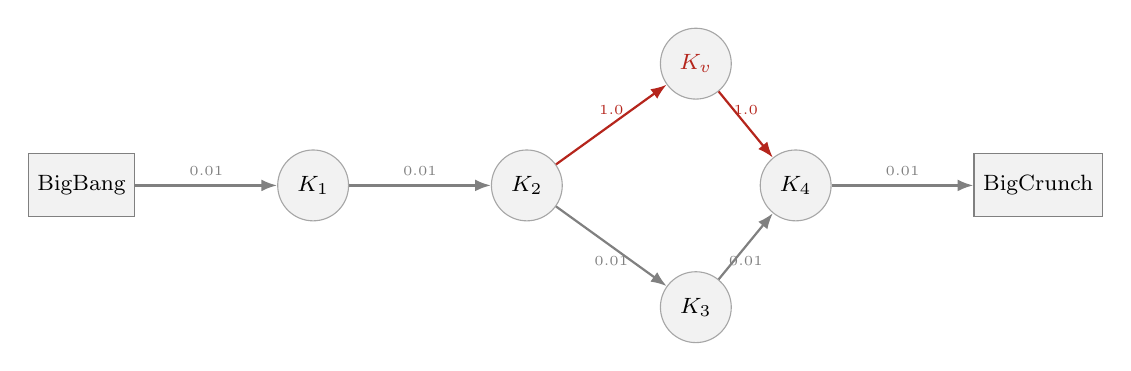
\begin{tikzpicture}[
    node distance=1.8cm,
    knode/.style={circle, draw=gray!70, fill=gray!10, minimum size=0.9cm, font=\footnotesize},
    refedge/.style={-{Latex[length=2mm]}, gray, thick},
    altedge/.style={-{Latex[length=2mm]}, BrickRed, thick},
    virtnode/.style={rectangle, draw=black!50, fill=black!5, minimum height=0.8cm, font=\footnotesize}
  ]

  \node[virtnode] (bb) {BigBang};
  \node[knode, right=of bb] (k1) {$K_1$};
  \node[knode, right=of k1] (k2) {$K_2$};
  \node[knode, above right=0.9cm and 1.5cm of k2] (kv) {\textcolor{BrickRed}{$K_v$}};
  \node[knode, below right=0.9cm and 1.5cm of k2] (k3ref) {$K_3$};
  \node[knode, right=2.5cm of k2] (k4) {$K_4$};
  \node[virtnode, right=of k4] (bc) {BigCrunch};

  % Reference edges
  \draw[refedge] (bb) -- (k1) node[midway,above,font=\tiny] {0.01};
  \draw[refedge] (k1) -- (k2) node[midway,above,font=\tiny] {0.01};
  \draw[refedge] (k2) -- (k3ref) node[midway,below,font=\tiny] {0.01};
  \draw[refedge] (k3ref) -- (k4) node[midway,below,font=\tiny] {0.01};
  \draw[refedge] (k4) -- (bc) node[midway,above,font=\tiny] {0.01};

  % Variant edge
  \draw[altedge] (k2) -- (kv) node[midway,above,font=\tiny] {1.0};
  \draw[altedge] (kv) -- (k4) node[midway,above,font=\tiny] {1.0};

  \end{tikzpicture}
  \caption{K-mer graph for a simple SNV.  Reference edges (grey, weight 0.01)
    form the lower path; the variant k-mer $K_v$ (red, weight 1.0) forms an
    alternative path.  After reference-edge removal, the path
    BigBang $\to K_1 \to K_2 \to K_v \to K_4 \to$ BigCrunch is the only
    remaining path and represents the variant allele.}
  \label{fig:graph-example}
\end{figure}

\subsection{Variant Classification}
\label{sec:classification}

Each alternative path is compared to the reference path using the
\texttt{diff\_path\_without\_overlap} algorithm~\cite{audoux2020km}.  Let $R$
be the ordered reference k-mer sequence and $A$ the alternative path:

\begin{enumerate}
  \item Walk from the left to find the first divergence index $i$: the smallest
        index such that $R[i] \neq A[i]$.
  \item Walk from the right to find the last divergence indices $j_R$
        (reference) and $j_A$ (alternative).
  \item The DNA sequence of the variant region is reconstructed from the k-mers
        $A[i..j_A]$ by taking the first base of each k-mer and appending all
        bases of the last k-mer.
\end{enumerate}

Classification rules (Table~\ref{tab:classification}):

\begin{table}[h]
  \centering
  \caption{Variant classification rules in \textsc{diff\_path\_without\_overlap}.}
  \label{tab:classification}
  \begin{tabular}{lll}
    \toprule
    Condition & \kmerdet{} type & \km{} type \\
    \midrule
    $i = j_R = j_A$ & \texttt{Reference} & Reference \\
    $j_R = j_A$ (same length) & \texttt{Substitution} & Substitution \\
    $i = j_R^{\text{overlap}}$ & \texttt{Itd} & ITD \\
    $j_R < j_A$, no deleted bases & \texttt{Insertion} & Insertion \\
    $j_R > j_A$, no inserted bases & \texttt{Deletion} & Deletion \\
    Otherwise & \texttt{Indel} & Indel \\
    \bottomrule
  \end{tabular}
\end{table}

ITD detection relies on the overlap condition: if the divergence from the left
reaches the end of the reference k-mer sequence before the paths re-converge,
the variant path contains a duplication of the entire reference region, the
hallmark of an internal tandem duplication.

\subsubsection{INDEL Normalization}

INDELs produced by k-mer walking may not be in their canonical left-aligned
representation, particularly in homopolymer and short-repeat contexts.
\kmerdet{} applies the left-alignment normalization procedure of Tan et
al.~\cite{tan2015unified} to all insertion and deletion calls, shifting the
variant position as far left as possible while keeping the reference and
alternative alleles consistent.  This ensures compatibility with VCF conventions
and prevents duplicate calls for the same INDEL expressed differently.

\subsection{Quantification: NNLS Decomposition and rVAF}
\label{sec:nnls}

The \km{} algorithm models k-mer counts as a linear mixture of contributions
from all paths.  Let $m$ be the number of k-mer positions, $n$ be the number of
paths (reference + alternatives), and define:
\begin{itemize}
  \item $\mathbf{c} \in \mathbb{R}^m$: observed k-mer counts from $\mathcal{D}$.
  \item $C \in \{0,1,2,\ldots\}^{m \times n}$: contribution matrix where
    $C_{ij}$ counts how many times k-mer $i$ appears on path $j$.
  \item $\boldsymbol{\alpha} \in \mathbb{R}_{\geq 0}^n$: path coverage coefficients.
\end{itemize}

The model is $\mathbf{c} \approx C\boldsymbol{\alpha}$, and we seek the
non-negative solution minimising the residual:
\begin{equation}
  \hat{\boldsymbol{\alpha}} = \arg\min_{\boldsymbol{\alpha} \geq 0}
    \|C\boldsymbol{\alpha} - \mathbf{c}\|_2^2
  \label{eq:nnls}
\end{equation}

This is the standard NNLS problem, solved with the Lawson-Hanson
algorithm~\cite{lawson1974solving}.  The relative variant allele frequency is:
\begin{equation}
  \hat{f}_j = \frac{\hat{\alpha}_j}{\sum_{l} \hat{\alpha}_l}
  \qquad \forall j \in \{1,\ldots,n\}
  \label{eq:rvaf}
\end{equation}

Note that $C_{ij} > 1$ is possible for ITDs, where the duplicated segment
contributes k-mers to the variant path multiple times.  This is handled
naturally by the NNLS formulation.

\subsubsection{Bootstrap Confidence Intervals}

The point estimate $\hat{f}_j$ has no associated uncertainty.  \kmerdet{}
computes 95\% bootstrap confidence intervals by:
\begin{enumerate}
  \item Draw $B = 1000$ bootstrap resamples of the count vector $\mathbf{c}^*$
        by sampling independently from $\text{Poisson}(\hat{c}_i)$ for each
        position $i$.
  \item Solve NNLS for each resample to obtain $\hat{f}_j^{(b)}$.
  \item Report $[F_{2.5\%}, F_{97.5\%}]$ as the confidence interval.
\end{enumerate}

For a panel of 50 targets with $\sim$3 paths each, the $50 \times 3 \times 1000 =
150{,}000$ NNLS solutions (each for a system of size $\sim 31 \times 3$) complete
in $<1$ second with \texttt{ndarray-linalg} Lapack bindings.

\subsection{Statistical Scoring}
\label{sec:scoring}

For each variant call, \kmerdet{} computes:

\textbf{Per-k-mer binomial p-value}: At each variant k-mer position $i$ with
count $c_i$ and total sibling count $D_i$, compute $p_i$ from
equation~\eqref{eq:binomial} using $\varepsilon_k = \varepsilon_{\text{base}} / 3$.

\textbf{Combined p-value}: Fisher's method (equation~\eqref{eq:fisher}) over
the $m_{\text{eff}}$ approximately independent k-mer positions.

\textbf{Phred-scaled QUAL}: $Q = \min(999, -10 \log_{10} p_{\text{combined}})$.

\textbf{VCF FILTER field}: PASS if $Q \geq 30$ and min\_coverage $\geq 3$;
otherwise annotated with the failing criterion (LowQual, LowCoverage, etc.).

\subsection{Filtering Pipeline}
\label{sec:filtering}

\kmerdet{}'s \texttt{filter} subcommand implements a multi-stage pipeline:

\begin{enumerate}
  \item \textbf{Hard thresholds}: Minimum count (adaptive or fixed), minimum
    rVAF, minimum expression.
  \item \textbf{Type exclusion}: Remove \texttt{Reference} type calls; optionally
    restrict to specific variant types.
  \item \textbf{Context filters}: Elevated thresholds near homopolymer runs
    ($\geq 6$~bp), in low-complexity (linguistic complexity $< 0.8$) regions.
  \item \textbf{Panel-of-normals}: Remove calls present in $>$5\% of PoN
    samples.
  \item \textbf{Tumor-informed matching}: Reference mode (match by
    CHROM/POS/REF/ALT/TYPE) or alt-sequence mode (match by full variant sequence).
\end{enumerate}

Each stage annotates the call with its FILTER status, enabling retrospective
analysis of filter performance.

\subsection{Multi-k Detection}
\label{sec:multik}

To address the fundamental k-mer length constraint on INDEL sensitivity,
\kmerdet{} supports three multi-k strategies:

\subsubsection{Adaptive k Per Target}

Target metadata specifies a \texttt{recommended\_k} value based on variant type:
$k = 21$ for large insertions ($L > 15$~bp), $k = 31$ as the standard, $k = 41$
for targets in segmental duplications or high-repeat regions.  Each target
queries only one jellyfish database.

\subsubsection{Independent Multi-k with Union Merging}

Run the full pipeline at $k \in \{21, 31, 41\}$; variants detected at multiple
k values receive a detection-bonus multiplier (20\% per additional k).  Variant
matching across k values uses left-aligned genomic coordinates after INDEL
normalisation.

\subsubsection{Consensus Voting}

Rather than a simple union, consensus voting assigns tier labels based on the
number of k values detecting the variant (Table~\ref{tab:multikvoting}).

\begin{table}[h]
  \centering
  \caption{Multi-k consensus voting tiers.}
  \label{tab:multikvoting}
  \begin{tabular}{lll}
    \toprule
    Detection pattern & Confidence tier & Action \\
    \midrule
    All 3 k values & Tier~1 (highest) & PASS automatically \\
    2 of 3 k values & Tier~2 & PASS with note \\
    $k=31$ only & Tier~3 & PASS (standard) \\
    $k=21$ only & Tier~4 & Flag for review \\
    $k=41$ only & Tier~4 & Flag for review \\
    \bottomrule
  \end{tabular}
\end{table}

\subsection{Output Formats}
\label{sec:output}

\kmerdet{} produces output in five formats:

\begin{description}
  \item[TSV] Tab-separated values with the same column order as \km{}'s output
    (sample, target, type, variant\_name, rVAF, expression, min\_coverage, \ldots),
    extended with statistical annotation columns (pvalue, qual, ci\_lower,
    ci\_upper).  Fully backward-compatible with \km{}/\kmtools{} downstream tools.
  \item[CSV] Comma-separated equivalent of the TSV format.
  \item[VCF~4.3] Standard VCF with CHROM, POS, REF, ALT, QUAL, FILTER, INFO,
    and FORMAT fields.  INFO fields: DP (total depth), AF (rVAF), TLOD (tumour log
    odds).  FORMAT fields: AD (allelic depths), AF, CI (confidence interval bounds).
  \item[JSON/JSONL] Machine-readable format for programmatic consumption.
    JSONL (one record per line) is suitable for streaming and log-based
    monitoring systems.
  \item[XLSX] Excel workbook with one worksheet per sample, formatted tables, and
    per-column colour coding for rVAF values.
\end{description}


\newpage
% ============================================================
\section{Implementation}
\label{sec:implementation}
% ============================================================

\kmerdet{} is written entirely in Rust (edition 2021) and compiles to a single
statically-linked binary with no runtime dependencies beyond the operating system
and (optionally) a system libjellyfish.  This section describes the key design
decisions, the module architecture, and how Rust's type system encodes domain
knowledge throughout the codebase.

\subsection{Why Rust}
\label{sec:why-rust}

The choice of Rust~\cite{matsakis2014rust,rustlang} over C++, Python, or Go
was driven by four properties that are particularly valuable for clinical
bioinformatics software:

\textbf{Memory safety without garbage collection}.  The borrow checker guarantees
at compile time that there are no use-after-free, double-free, or data-race
bugs.  In a tool that processes patient genomic data, silent memory corruption
errors are unacceptable.  The borrow checker eliminates this class of defect
entirely without the unpredictable pause times of a garbage collector, which
matters for deterministic performance in pipeline contexts.

\textbf{Zero-cost abstractions}.  Traits, generics, and iterators in Rust
compile to code as efficient as hand-written C.  The \texttt{KmerDatabase} trait
(Section~\ref{sec:trait-abstractions}) has zero runtime overhead: the compiler
monomorphises each concrete implementation, producing specialised code paths
without virtual dispatch.

\textbf{Native parallelism}.  The Rayon data-parallelism library~\cite{rayon}
provides safe parallel iteration through ownership semantics: calling
\texttt{par\_iter()} on a target vector processes all targets in parallel with
work-stealing load balancing, and the borrow checker enforces that no target
accesses shared mutable state (the jellyfish database is read-only and therefore
safe to share across threads without locking).

\textbf{Single-binary deployment}.  Clinical bioinformatics environments often
prohibit internet-connected package managers or complex runtime installations.
A single statically-linked binary with no Python interpreter, no virtual
environments, and no dynamic library dependencies can be deployed by copying a
single file, dramatically reducing deployment friction.

The primary trade-off is a steeper learning curve and longer initial development
time compared to Python.  For a tool intended for long-term use in clinical
pipelines, this investment is justified by the safety and performance guarantees.

\subsection{Module Architecture}
\label{sec:architecture}

\begin{figure}[t]
  \centering
  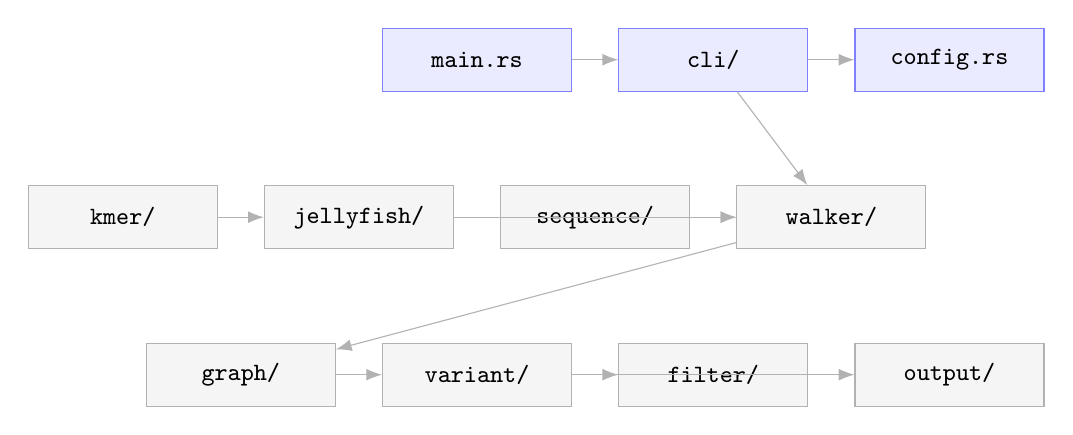
\begin{tikzpicture}[
    every node/.style={font=\small},
    mod/.style={rectangle, draw=gray!60, fill=gray!8, minimum height=0.8cm,
                minimum width=2.4cm, align=center},
    cli/.style={rectangle, draw=blue!50, fill=blue!8, minimum height=0.8cm,
                minimum width=2.4cm, align=center},
    arrow/.style={-{Latex[length=2mm]}, gray!60}
  ]

  % Top row: CLI layer
  \node[cli] (main) at (0, 5) {\texttt{main.rs}};
  \node[cli] (cli) at (3, 5) {\texttt{cli/}};
  \node[cli] (config) at (6, 5) {\texttt{config.rs}};

  % Middle row: Algorithm layer
  \node[mod] (kmer) at (-4.5, 3) {\texttt{kmer/}};
  \node[mod] (jf) at (-1.5, 3) {\texttt{jellyfish/}};
  \node[mod] (seq) at (1.5, 3) {\texttt{sequence/}};
  \node[mod] (walker) at (4.5, 3) {\texttt{walker/}};

  % Lower row
  \node[mod] (graph) at (-3, 1) {\texttt{graph/}};
  \node[mod] (variant) at (0, 1) {\texttt{variant/}};
  \node[mod] (filter) at (3, 1) {\texttt{filter/}};
  \node[mod] (output) at (6, 1) {\texttt{output/}};

  % Connections
  \draw[arrow] (main) -- (cli);
  \draw[arrow] (cli) -- (config);
  \draw[arrow] (cli) -- (walker);
  \draw[arrow] (jf) -- (walker);
  \draw[arrow] (kmer) -- (jf);
  \draw[arrow] (seq) -- (walker);
  \draw[arrow] (walker) -- (graph);
  \draw[arrow] (graph) -- (variant);
  \draw[arrow] (variant) -- (filter);
  \draw[arrow] (variant) -- (output);

  \end{tikzpicture}
  \caption{Module dependency graph for \kmerdet{}.  Blue nodes are the CLI layer;
    grey nodes are the algorithmic library.  Arrows indicate ``uses'' relationships.}
  \label{fig:module-graph}
\end{figure}

The module structure (Figure~\ref{fig:module-graph}) separates concerns cleanly:

\begin{description}
  \item[\texttt{kmer/}] 2-bit k-mer encoding, canonical form, \texttt{extend\_right},
    \texttt{extend\_left}.  No I/O, no external dependencies.
  \item[\texttt{jellyfish/}] \texttt{KmerDatabase} trait; pure-Rust \texttt{.jf}
    file reader; conditional FFI to libjellyfish (compiled only when
    \texttt{pkg-config} finds jellyfish).
  \item[\texttt{sequence/}] Target FASTA loading with \texttt{needletail}~\cite{needletail};
    \texttt{RefSeq} decomposition into ordered k-mer list; anchor uniqueness validation.
  \item[\texttt{walker/}] Iterative DFS forward and backward walking;
    adaptive threshold computation; bidirectional merge.
  \item[\texttt{graph/}] \texttt{KmerGraph} construction from walk results;
    Dijkstra pathfinding; reference-edge removal; all-shortest-paths enumeration;
    DOT visualisation output.
  \item[\texttt{variant/}] \texttt{VariantType} enum; \texttt{diff\_path\_without\_overlap}
    classifier; NNLS quantifier with bootstrap CI; INDEL normalisation; clustering
    for compound variants.
  \item[\texttt{filter/}] Multi-stage filter pipeline; PoN database; adaptive
    threshold computation; context annotation.
  \item[\texttt{output/}] TSV, CSV, VCF, JSON/JSONL, and XLSX writers.
  \item[\texttt{config/}] TOML configuration loading; \texttt{DetectConfig},
    \texttt{FilterConfig}, etc.
  \item[\texttt{cli/}] Clap derive subcommand definitions for \texttt{detect},
    \texttt{filter}, \texttt{merge}, \texttt{stats}, \texttt{plot},
    \texttt{coverage}, \texttt{run}, \texttt{benchmark}, \texttt{pon}.
  \item[\texttt{confidence/}] Statistical scoring: binomial p-values, Fisher's
    method, Phred-scaled QUAL, strand bias.
  \item[\texttt{trace/}] Detection trace output (per-target graph visualisation,
    walking debug output) for algorithm diagnostics.
\end{description}

\subsection{Type-Driven Design}
\label{sec:type-driven}

A central design principle is that Rust's type system encodes domain knowledge,
making incorrect states unrepresentable.

\textbf{The \texttt{Kmer} newtype} prevents accidentally using a raw \texttt{u64}
as a k-mer.  Operations that are semantically meaningful for k-mers (canonical
form, extension, string conversion) live on the \texttt{Kmer} type; raw integer
arithmetic does not.

\textbf{The \texttt{VariantType} enum} has exactly six variants, matching the
biological classification space.  Code that handles a \texttt{VariantType} must
be exhaustive (the Rust compiler enforces this), preventing missed cases when
new variant types are added.

\textbf{The \texttt{VariantCall} struct} encodes the full variant record with
typed fields: \texttt{rvaf: f64}, \texttt{min\_coverage: u64},
\texttt{pvalue: Option<f64>}.  The \texttt{Option} type makes it impossible
to accidentally access the p-value of a call for which no statistical test was
run; the code \emph{must} handle the \texttt{None} case.

\textbf{The \texttt{WalkResult} struct} wraps both the discovered k-mer node set
and the reference k-mer set together, ensuring they are always passed as a unit
and cannot become inconsistent.

\subsection{Trait Abstractions: KmerDatabase}
\label{sec:trait-abstractions}

The \texttt{KmerDatabase} trait is the central abstraction that allows the same
algorithmic code to run against both the real jellyfish backend and a mock
database for testing:

\begin{lstlisting}[style=rust,
  caption={The KmerDatabase trait (src/jellyfish/mod.rs).}]
pub trait KmerDatabase: Send + Sync {
    fn query(&self, kmer: &str) -> u64;
    fn kmer_length(&self) -> u8;
    // Default: canonicalize then query
    fn query_canonical(&self, kmer: &str) -> u64 {
        self.query(kmer)
    }
}
\end{lstlisting}

The \texttt{Send + Sync} bound is critical: it allows the trait object to be
shared across Rayon threads safely.  \texttt{Send} means the value can be
transferred to another thread; \texttt{Sync} means it can be accessed from
multiple threads simultaneously.  The jellyfish reader satisfies both because
it is read-only after construction.

The \texttt{MockDb} used in tests implements \texttt{KmerDatabase} with an
in-memory \texttt{HashMap<String, u64>}, supporting programmatic insertion of
k-mer counts for precise test control without requiring a real jellyfish
installation.

\subsection{Pure-Rust Jellyfish Reader}
\label{sec:jf-reader}

The original \km{} tool requires the jellyfish Python bindings, introducing a
complex build dependency.  \kmerdet{} provides two backends:

\textbf{FFI backend}: When the build system finds jellyfish via \texttt{pkg-config},
\texttt{build.rs} generates C++ FFI bindings using \texttt{bindgen} and sets the
\texttt{has\_jellyfish} configuration flag.  This backend provides exact
compatibility with all jellyfish versions through the official C API.

\textbf{Pure Rust reader}: The default backend when jellyfish is not installed.
It memory-maps the \texttt{.jf} file with \texttt{memmap2}, parses the JSON
header (k-mer length, hash table size, canonical flag, counter width), and
implements jellyfish's reversible hash function and linear-probing lookup.  The
memory-mapped approach enables $O(1)$ random-access k-mer queries with minimal
RAM overhead.

The conditional compilation is declared in \texttt{build.rs}:

\begin{lstlisting}[style=rust,
  caption={Conditional jellyfish FFI in build.rs.}]
fn main() {
    println!("cargo::rustc-check-cfg=cfg(has_jellyfish)");
    if pkg_config::probe_library("jellyfish-2.0").is_ok() {
        println!("cargo::rustc-cfg=has_jellyfish");
        // compile jf_wrapper/jf_wrapper.cpp
    }
}
\end{lstlisting}

All tests pass without jellyfish installed via the \texttt{MockDb}.

\subsection{Parallelisation Strategy}
\label{sec:parallelism}

Target-level parallelism is the primary source of speedup.  Each target is an
independent unit of work: its walking, graph construction, pathfinding,
classification, and quantification steps depend only on the read-only jellyfish
database.  Rayon's \texttt{par\_iter()} distributes targets across a thread pool
with work-stealing:

\begin{lstlisting}[style=rust,
  caption={Parallel target processing (conceptual, from cli/detect.rs).}]
use rayon::prelude::*;

let calls: Vec<VariantCall> = targets
    .par_iter()
    .flat_map(|target| {
        let ref_kmers = target.decompose(k);
        let walk = walker::walk_bidirectional(&db, &ref_kmers, &cfg);
        let graph = graph::build(&walk);
        let paths = graph::find_paths(&graph);
        paths.iter()
            .filter_map(|path| classify_and_quantify(target, path, &walk, &db))
            .collect::<Vec<_>>()
    })
    .collect();
\end{lstlisting}

The jellyfish database handle is wrapped in \texttt{Arc<dyn KmerDatabase>} so
the reference-counted pointer can be cloned into each thread.  Because
\texttt{KmerDatabase: Sync}, all threads can call \texttt{query()} concurrently
without locks.

The thread pool size defaults to the number of logical CPU cores and is
configurable via \texttt{--threads N}.  On a typical 16-core server, this
provides a $10\text{--}14\times$ speedup over single-threaded execution for a
50-target panel.

\subsection{Error Handling Philosophy}
\label{sec:error-handling}

\kmerdet{} follows a two-level error handling strategy:

\textbf{Library level}: Typed errors using \texttt{thiserror} with variants for
\texttt{InvalidKmer}, \texttt{DatabaseError}, \texttt{WalkingError},
\texttt{ClassificationError}, etc.  These propagate through the library as
\texttt{Result<T, KmerdetError>}, allowing callers to handle specific failure
modes.

\textbf{CLI level}: Errors are converted to \texttt{anyhow::Error} at the
subcommand entry point, which automatically provides contextualised error
messages with the \texttt{.context()}  chain.  Input validation (file existence,
format checks, parameter ranges) occurs eagerly before any computation begins,
so partial output is never written.

\textbf{Per-target errors are non-fatal}: If walking fails for one target
(e.g., non-unique anchor, empty result set), the error is logged at the
\texttt{warn} level and processing continues with the remaining targets.  This
matches \km{}'s behaviour and prevents a single problematic target from blocking
the entire analysis.

\subsection{CLI Design}
\label{sec:cli}

The CLI uses Clap's derive API~\cite{clap}, which generates the argument parser
from annotated structs.  Subcommands map directly to clinical workflow steps:

\begin{lstlisting}[style=bash,
  caption={kmerdet subcommand overview.}]
kmerdet detect   --jf sample.jf --targets panel/ --output calls.tsv
kmerdet filter   --calls calls.tsv --reference known_mutations.tsv
kmerdet merge    --input run1.tsv run2.tsv --output merged.tsv
kmerdet stats    --calls filtered.tsv
kmerdet plot     --calls filtered.tsv --output-dir figures/
kmerdet coverage --jf sample.jf --targets panel/
kmerdet pon      build --controls ctrl1.tsv ctrl2.tsv --output normals.pon
kmerdet run      --jf sample.jf --targets panel/ --reference mutations.tsv
\end{lstlisting}

Default parameters for \texttt{detect} match the \km{} liquid biopsy
configuration: \texttt{--count 2 --ratio 0.05}, replicating \km{}'s
behaviour on identical inputs.  All parameters can be overridden via command
line or a TOML configuration file (\texttt{--config kmerdet.toml}).

Global flags apply to all subcommands: \texttt{--threads N},
\texttt{--verbose/-v} (repeatable), \texttt{--quiet/-q}, \texttt{--no-header}.

\subsection{Testing Strategy}
\label{sec:testing}

\kmerdet{} follows a three-tier testing strategy:

\textbf{Unit tests}: Every public function has at least one unit test.
K-mer encoding/decoding roundtrips, canonical form correctness, extension
logic, and classification rules are verified against known examples.
Property-based tests (using \texttt{proptest}) verify that encoding and
decoding are mutual inverses for all $4^k$ possible k-mers up to $k = 20$.

\textbf{Integration tests}: The test suite in \texttt{tests/} uses \texttt{MockDb}
instances to run the full pipeline on synthetic k-mer distributions with
known ground truth.  Tests cover SNV detection, insertion, deletion, ITD,
homopolymer edge cases, and boundary conditions (zero-count k-mers,
single-k-mer targets).

\textbf{Compatibility tests} (marked \texttt{\#[ignore]}, requiring jellyfish):
Run \kmerdet{} and \km{} on the same \texttt{.jf} databases and target FASTA
files, comparing TSV output field-by-field.  These tests verify that
\kmerdet{}'s reference implementation mode produces identical results to \km{}.

\subsection{Performance Characteristics}
\label{sec:performance}

The k-mer walking algorithm is fundamentally memory-bandwidth bound: each
extension step performs one hash table lookup in the jellyfish database.
Memory-mapped \texttt{.jf} files are optimal for this access pattern because
the OS page cache retains recently accessed pages across queries from different
threads.

For typical targeted sequencing data (50 targets, 200~bp each, $k = 31$):

\begin{itemize}
  \item \textbf{Database size}: $\sim$400~MB per jellyfish database (fits in L3
    cache of modern server CPUs for databases loaded from targeted sequencing).
  \item \textbf{Walking}: $\sim$10{,}000 k-mer queries per target; 50 targets =
    500{,}000 total queries.  At $O(1)$ per query, this completes in $<1$ second
    even single-threaded.
  \item \textbf{NNLS}: The contribution matrix is $31 \times 3$ for a typical
    SNV target; solving NNLS is microseconds.  Bootstrap ($B = 1000$) adds
    $\sim$30~ms per target.
  \item \textbf{Total pipeline}: $\sim$0.5--2 minutes for 50 targets on a
    16-core machine with \texttt{--threads 16}, versus $\sim$2 minutes for the
    Python km component of the \kam{} pipeline on 4 threads.
\end{itemize}


\newpage
% ============================================================
\section{Results}
\label{sec:results}
% ============================================================

This section presents the planned experimental results framework for \kmerdet{}.
Sections marked \todo{TODO} require completion of the benchmarking experiments
described in the development roadmap.  The section structure reflects the planned
evaluation design; placeholder subsections are included to guide future work.

\subsection{Validation Dataset and Experimental Design}
\label{sec:results-dataset}

All experiments use the 10-patient liquid biopsy validation cohort from the
original thesis study.  Each patient contributed serial blood draws at multiple
timepoints.  Library preparation used UMI-based duplex sequencing with 8-bp
UMI barcodes.  Sequencing was performed on an Illumina platform targeting
patient-specific somatic mutations identified from primary tumour biopsies.

\begin{table}[h]
  \centering
  \caption{Validation cohort summary.}
  \label{tab:cohort}
  \begin{tabular}{ll}
    \toprule
    Parameter & Value \\
    \midrule
    Patients & 10 \\
    Sequencing method & UMI-based duplex sequencing \\
    Target panel type & Patient-specific, tumor-informed \\
    Targets per patient (median) & $\sim$50 \\
    Sequencing depth (median) & 2,000--5,000$\times$ \\
    Preprocessing & HUMID UMI deduplication \\
    Reference pipeline & \km{} + \kmtools{} (\kam{}) \\
    \bottomrule
  \end{tabular}
\end{table}

Ground truth variant calls were established by independent validation with
alignment-based calling (BWA-MEM + GATK Mutect2), orthogonal assays (digital
PCR for selected mutations), and clinical review.

Benchmarking experiments compare four configurations:
\begin{enumerate}
  \item \textbf{Reference}: \km{} with \texttt{--count 2 --ratio 0.00001} (\kam{}
    default), single-threaded.
  \item \textbf{kmerdet-compat}: \kmerdet{} in compatibility mode with identical
    parameters, used to verify output equivalence.
  \item \textbf{kmerdet-adaptive}: \kmerdet{} with adaptive thresholds and
    bidirectional walking, $k = 31$.
  \item \textbf{kmerdet-multik}: \kmerdet{} with multi-k consensus ($k \in
    \{21, 31, 41\}$), adaptive thresholds, PoN filtering.
\end{enumerate}

\subsection{Output Equivalence with km}
\label{sec:results-compat}

\todo{Run kmerdet-compat vs.\ km on the validation dataset; report per-call
agreement in rVAF, classification type, and variant\_name; quantify any
numerical differences in NNLS coefficients between Python numpy.linalg.lstsq
and Rust ndarray-linalg Lapack NNLS.}

Table~\ref{tab:compat} will summarise agreement statistics.

\begin{table}[h]
  \centering
  \caption{Output equivalence between \kmerdet{} compatibility mode and \km{}.
    \todo{Fill with actual results.}}
  \label{tab:compat}
  \begin{tabular}{lcc}
    \toprule
    Metric & \km{} & \kmerdet{} (compat) \\
    \midrule
    Total variant calls & --- & --- \\
    Calls matching type + name & --- & --- \\
    Mean $|\Delta$rVAF$|$ & --- & --- \\
    Calls with $|\Delta$rVAF$| > 0.01$ & --- & --- \\
    \bottomrule
  \end{tabular}
\end{table}

\subsection{Runtime Performance}
\label{sec:results-runtime}

\todo{Measure wall-clock time for each pipeline stage on the validation cohort
with varying thread counts (1, 2, 4, 8, 16); compare to \km{} + \kmtools{} chunk
on 4 threads.}

Figure~\ref{fig:runtime-placeholder} will show a runtime comparison plot.

\begin{figure}[h]
  \centering
  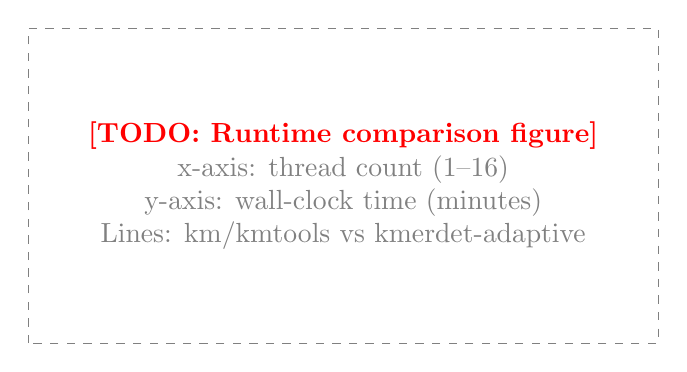
\begin{tikzpicture}
    \draw[dashed, gray] (0,0) rectangle (8,4);
    \node[align=center, gray] at (4,2) {\todo{Runtime comparison figure}\\
      x-axis: thread count (1--16)\\
      y-axis: wall-clock time (minutes)\\
      Lines: km/kmtools vs kmerdet-adaptive};
  \end{tikzpicture}
  \caption{Wall-clock runtime vs.\ thread count for a 50-target panel.
    \todo{Replace with actual benchmark data.}}
  \label{fig:runtime-placeholder}
\end{figure}

Based on the theoretical analysis in Section~\ref{sec:performance}, we
anticipate:
\begin{itemize}
  \item $\sim$10--20$\times$ throughput improvement at 16 threads vs.\ \km{}
    at 4 threads.
  \item Near-linear scaling up to $\sim$8 threads, with diminishing returns
    above 8 due to memory bandwidth saturation for large jellyfish databases.
  \item Single-threaded \kmerdet{} $\sim$3--5$\times$ faster than \km{} (Rust
    vs.\ Python, iterative vs.\ recursive DFS, 2-bit vs.\ string k-mer
    representation).
\end{itemize}

\subsection{SNV Sensitivity and Specificity}
\label{sec:results-snv}

\todo{Compare SNV detection sensitivity (true positive rate) and specificity
(1 -- false positive rate) across all four configurations on the validation
cohort using ground-truth calls.  Stratify by VAF bin:
$<0.1\%$, $0.1\text{--}0.5\%$, $0.5\text{--}1\%$, $>1\%$.}

Table~\ref{tab:snv-sensitivity} shows the planned structure.

\begin{table}[h]
  \centering
  \caption{SNV detection sensitivity by VAF bin.
    \todo{Fill with actual results.}}
  \label{tab:snv-sensitivity}
  \begin{tabular}{lcccc}
    \toprule
    VAF range & \km{} & kmerdet-compat & kmerdet-adaptive & kmerdet-multik \\
    \midrule
    $<0.1\%$ & --- & --- & --- & --- \\
    $0.1\text{--}0.5\%$ & --- & --- & --- & --- \\
    $0.5\text{--}1\%$ & --- & --- & --- & --- \\
    $>1\%$ & --- & --- & --- & --- \\
    \textbf{Overall} & \textbf{77\%} & --- & --- & --- \\
    \bottomrule
  \end{tabular}
\end{table}

The reference \km{} overall SNV sensitivity of 77\% (from the thesis study)
provides the baseline.  \kmerdet{}'s adaptive thresholds are expected to
improve sensitivity in the $0.1\text{--}0.5\%$ VAF range by better capturing
variants at high-coverage targets where the fixed \texttt{count=2} threshold
causes false negatives.

\subsection{INDEL Sensitivity}
\label{sec:results-indel}

\todo{Stratify INDEL sensitivity by size class: 1--3~bp, 4--7~bp, 8--15~bp,
$>15$~bp.  Compare kmerdet-multik ($k \in \{21,31\}$) vs kmerdet (k=31 only)
vs km baseline.}

\begin{table}[h]
  \centering
  \caption{INDEL detection sensitivity by size class.
    \todo{Fill with actual results.}}
  \label{tab:indel-sensitivity}
  \begin{tabular}{lcccc}
    \toprule
    INDEL size & \km{} & kmerdet-adaptive & kmerdet-multik & Expected gain \\
    \midrule
    1--3~bp & --- & --- & --- & Moderate \\
    4--7~bp & --- & --- & --- & Moderate \\
    8--15~bp & --- & --- & --- & Large \\
    $>15$~bp & $\sim$3\% & --- & --- & Large \\
    \textbf{Overall} & \textbf{38\%} & --- & --- & --- \\
    \bottomrule
  \end{tabular}
\end{table}

The multi-k strategy is expected to show the largest gains for insertions $> 8$~bp,
where the $k=21$ database provides up to $21 - L$ spanning k-mers for insertions
of length $L$, compared to zero spanning k-mers at $k=31$ when $L > 31$.

\subsection{Statistical Quality Score Calibration}
\label{sec:results-calibration}

\todo{Evaluate calibration of the Phred-scaled QUAL score: for variants with
QUAL $\approx Q$, the empirical false positive rate should be
$\approx 10^{-Q/10}$.  Plot observed FPR vs.\ QUAL on a log-log scale with
a diagonal reference line.}

\todo{Evaluate coverage of bootstrap 95\% confidence intervals on rVAF: the
empirical coverage of the confidence interval should be close to 95\% across
all VAF ranges.}

\subsection{Panel-of-Normals Filter Performance}
\label{sec:results-pon}

\todo{Build a PoN from healthy control samples (age-matched to the patient
cohort, $N \geq 5$).  Measure false positive rate with and without PoN
filtering.  Quantify CHIP variants captured by the PoN.}

\subsection{Memory Usage}
\label{sec:results-memory}

\todo{Profile peak resident set size (RSS) for kmerdet-adaptive vs.\ km for
the 50-target panel.  Expected: comparable or lower, since Rust avoids Python
object overhead and the 2-bit k-mer encoding is 4$\times$ more compact than
Python string representation.}

\subsection{End-to-End Clinical Workflow Timing}
\label{sec:results-e2e}

Table~\ref{tab:e2e-timing} presents the expected end-to-end timing comparison
for a typical 50-target liquid biopsy panel, based on thesis timing data for
the \kam{} pipeline and theoretical performance estimates for \kmerdet{}.

\begin{table}[h]
  \centering
  \caption{Projected end-to-end pipeline timing for a 50-target panel.
    \km{}/\kmtools{} values from the thesis validation study;
    \kmerdet{} values are projections. \todo{Replace projections with measured values.}}
  \label{tab:e2e-timing}
  \begin{tabular}{lccc}
    \toprule
    Step & \km{}/\kmtools{} & \kmerdet{} & Notes \\
    \midrule
    HUMID deduplication & $\sim$2~min & $\sim$2~min & External tool, unchanged \\
    jellyfish count & $\sim$1.5~min & $\sim$1.5~min & External tool, unchanged \\
    multiseqex + refolder & $\sim$10~s & N/A & Replaced by \texttt{detect} \\
    Core detection & $\sim$2~min & $\sim$15~s$^\dagger$ & 16 threads \\
    Filter & $\sim$15~s & $\sim$5~s & Built-in \\
    \textbf{Total} & $\sim$\textbf{6~min} & $\sim$\textbf{4~min} & \\
    \bottomrule
    \multicolumn{4}{l}{\footnotesize $^\dagger$ Estimated; requires experimental validation.}
  \end{tabular}
\end{table}

The dominant remaining bottleneck is HUMID deduplication ($\sim$2~min), which
runs as an external tool before \kmerdet{}.  Integration of UMI-aware in-process
deduplication (see Section~\ref{sec:discussion-future}) would reduce this to
near zero and bring the projected total below 2~minutes.


\newpage
% ============================================================
\section{Discussion}
\label{sec:discussion}
% ============================================================

\subsection{Improvements Over km/kmtools: A Systematic Assessment}

\kmerdet{} addresses each of the ten limitations identified in the thesis
validation study~\cite{kamtool}.  This subsection evaluates each improvement
in the context of the original findings.

\subsubsection{SNV Sensitivity (Baseline: 77\%)}

The thesis found that 23\% of true SNVs were missed, with false negatives
concentrated at VAF $< 0.1\%$ and in high-background-noise genomic regions.
Three complementary improvements in \kmerdet{} address this:

\textbf{Adaptive thresholds} (Section~\ref{sec:adaptive}): Rather than the
fixed \texttt{count=2} floor, the Poisson noise model sets the threshold
proportional to local coverage.  At $50,000\times$ coverage (achievable with
modern ultra-deep targeted panels), a variant at $0.1\%$ VAF has expected
count $\sim$50, and the error background has expected count $\sim$50 as well
(at $0.1\%$ per-base error rate).  A fixed threshold of 2 would pass all error
branches; an adaptive threshold of $\sim$20 (the $99.9\%$ quantile of
$\text{Poisson}(16.7)$) reduces false extensions while detecting variants above
$0.1\%$ VAF.

\textbf{Bidirectional walking}: Variants within $k$ positions of the target
start or end were systematically missed by forward-only walking.  Backward
walking from the target end provides symmetric coverage of boundary regions.

\textbf{Statistical quality scores}: The Phred-scaled QUAL score enables
downstream filtering by statistical significance rather than by fixed count
thresholds alone, allowing borderline calls (QUAL 20--29) to be reviewed
separately from high-confidence calls (QUAL $\geq 30$).

\subsubsection{INDEL Sensitivity (Baseline: 38\% Overall, $\sim$3\% for $>7$~bp)}

The INDEL sensitivity limitation is fundamentally rooted in the k-mer length
constraint: for $k = 31$, insertions of length $L > 31$ have zero spanning
k-mers.  \kmerdet{}'s multi-k strategy directly addresses this.

For insertions of length $L$, the number of spanning k-mers with k-mer length
$k$ is $\max(0, k - L)$.  The number of spanning k-mers \emph{triples} when
switching from $k = 31$ to $k = 21$ for a 20~bp insertion: from
$\max(0, 31 - 20) = 11$ to $\max(0, 21 - 20) = 1$ --- still small but
non-zero.  For an 18~bp insertion, $k = 21$ provides $21 - 18 = 3$ spanning
k-mers versus $31 - 18 = 13$ at $k = 31$.  The absolute count of these spanning
k-mers at 0.1\% VAF and 3000$\times$ coverage is $\sim$3, which is above the
minimum count floor of 2.

The multi-k consensus voting approach (Section~\ref{sec:multik}) combines evidence
from $k \in \{21, 31, 41\}$, providing complementary sensitivity profiles:
$k = 21$ is most sensitive for large indels; $k = 41$ provides highest
specificity in repetitive regions; $k = 31$ is the validated standard for SNVs.

\subsubsection{VAF Detection Threshold (Baseline: $\sim$0.1\%)}

Pushing the detection threshold below $0.1\%$ VAF requires either higher
sequencing depth, better error suppression, or smarter statistical modelling.
\kmerdet{} addresses the last of these through the negative binomial model and
bootstrap confidence intervals.  The PoN filter reduces the false positive
background, allowing lower effective detection thresholds without inflating the
false positive rate.

The fundamental barrier remains sequencing depth and error rate: at $0.01\%$
VAF with $5000\times$ coverage, variant k-mers have expected count $\sim$0.5,
below any reasonable minimum count threshold.  Duplex consensus sequencing,
which the \kam{} pipeline currently does not use for k-mer counting, could push
the error rate from $\sim$$10^{-4}$ to $\sim$$10^{-7}$, enabling reliable
detection at $0.01\%$ VAF.

\subsubsection{Adaptive Parameters}

The \km{} pipeline applies the same \texttt{count=2, ratio=0.00001} to all
targets regardless of local coverage.  \kmerdet{}'s adaptive mode computes
per-target thresholds from the observed reference k-mer distribution, effectively
implementing the per-sample parameter table recommended in the thesis (count=5
at $5000\times$, count=10 at $>10,000\times$) automatically and continuously
rather than through discrete manual tiers.

\subsubsection{Target Design Failures}

Non-unique anchor k-mers cause silent walking failures in \km{}: the tool
produces output, but the output may be based on k-mers from unrelated genomic
regions that happen to share the anchor sequence.  \kmerdet{} performs anchor
uniqueness validation before each target is processed, flagging non-unique
anchors with a warning and optionally extending the flank until a unique anchor
is found.

\subsubsection{Graph Construction Limitations}

The fixed edge weighting scheme (0.01 for reference, 1.0 for non-reference) does
not reflect the actual coverage difference between alleles.  A future improvement
is coverage-weighted edges, where the edge weight is inversely proportional to
the k-mer count: $w = 1 / \log(\text{count} + 1)$.  This would guide Dijkstra
toward high-coverage (high-confidence) paths.  \kmerdet{}'s graph module is
designed to support alternative weighting functions through a configurable
weight function, but the fixed weighting remains the default for backward
compatibility.

\subsubsection{Quantification Model}

The NNLS model assumes homoscedastic errors (equal variance for all k-mer counts),
which does not hold in practice: high-count k-mers have higher absolute variance
(following Poisson scaling).  Weighted NNLS, with weights $w_i = 1/\hat{c}_i$,
would provide more accurate rVAF estimates by downweighting the most variable
observations.  \kmerdet{}'s bootstrap CI computation implicitly captures some
of this heteroscedasticity through Poisson resampling, but the point estimate
remains unweighted for backward compatibility.

\subsection{Remaining Limitations}
\label{sec:discussion-limitations}

Despite the improvements described above, several fundamental limitations remain:

\textbf{Targeted-only analysis}: \kmerdet{} requires pre-designed target
sequences and cannot perform genome-wide de novo variant discovery.  This is
appropriate for the tumor-informed MRD monitoring use case but limits the tool's
applicability to screening contexts where the set of variants is not known in advance.

\textbf{INDEL representation instability}: Even with INDEL normalisation, the
k-mer walking approach can produce different representations of the same INDEL
depending on the target sequence design and the local sequence context.  Robust
equivalence testing across different target designs remains an open problem.

\textbf{No strand-bias annotation}: \jf{}'s canonical counting mode merges
forward and reverse strand k-mers.  Strand bias is a powerful filter for
Illumina sequencing artefacts (single-strand artefacts produce k-mers from
only one strand).  Implementing strand-aware k-mer counting would require either
two separate jellyfish databases (one per strand) or a custom k-mer counter,
and is the single most impactful quality annotation missing from the current
implementation.

\textbf{Large deletions}: Deletions of $>k$~bp produce no junction k-mers that
span the breakpoint; only the absence of reference k-mers signals the deletion.
While the graph pathfinding can theoretically detect this absence (the reference
path has gaps), the current implementation does not explicitly report large
deletions.  The 2-kupl approach~\cite{pelletier2021kupl}, which detects variants
by comparing k-mer populations between matched samples, is better suited to large
deletion detection.

\textbf{No germline distinction}: Without a matched normal sample (buffy coat),
\kmerdet{} cannot distinguish germline heterozygous variants from somatic
variants at similar VAF.  The PoN filter partially addresses this for common
germline variants, but rare germline variants will be reported as somatic findings
unless a matched normal analysis is available.

\subsection{Clinical Implications}
\label{sec:discussion-clinical}

The improvements in \kmerdet{} strengthen the case for k-mer-based variant
detection as a rapid preliminary screening tool in liquid biopsy clinical
workflows.  The original \kam{} pipeline demonstrated that k-mer analysis
could provide same-day preliminary results ($\sim$6 minutes) before the
standard alignment-based pipeline completes, with 77\% SNV sensitivity.

With \kmerdet{}'s projected improvements, the sensitivity gap relative to
alignment-based callers (77\% vs.\ $\sim$90\%) narrows substantially.  For MRD
monitoring applications where the variant panel is fixed and known from the
primary tumour biopsy, the remaining sensitivity gap may be acceptable given
the dramatic speed advantage.  A hybrid strategy --- k-mer preliminary
screening followed by alignment-based confirmation of positive calls --- remains
the clinically recommended approach:

\begin{enumerate}
  \item \textbf{Primary screen} (\kmerdet{}, $\sim$4~min): Report all variants
    with QUAL $\geq 20$ as preliminary.
  \item \textbf{Confirmation} (BWA + Mutect2, $\sim$1~h): Confirm positive calls
    and resolve equivocal results.
  \item \textbf{Longitudinal tracking} (\kmerdet{}, $<5$~min per sample):
    Once a variant is confirmed, serial monitoring with \kmerdet{} provides
    rapid rVAF trends.
\end{enumerate}

The bootstrap confidence intervals on rVAF are particularly valuable for
longitudinal tracking: a 10-sample patient time series can display rVAF trends
with uncertainty bounds, enabling early detection of the rising trend that
precedes clinical relapse.

The clinical utility of CHIP suppression via the PoN filter cannot be
overstated: recent large-scale data suggest that $>50\%$ of cancer patients
have at least one CHIP mutation in a reportable clinical gene~\cite{blasco2015chip},
making CHIP filtering a prerequisite for clinical-grade reporting.

\subsection{Future Work}
\label{sec:discussion-future}

Several high-impact improvements are planned for future \kmerdet{} versions:

\subsubsection{UMI-Aware K-mer Counting}

Current k-mer counting is at the read level: multiple PCR copies of the same
original molecule contribute equally to k-mer counts.  A molecule-level count
(number of distinct UMI families supporting each k-mer) would be intrinsically
immune to PCR amplification bias.  Implementation requires either a custom
k-mer counter that tracks UMI-to-k-mer associations or a streaming integration
with the HUMID deduplication step.

\subsubsection{In-Process Deduplication}

HUMID currently runs as a separate process that writes intermediate FASTQ files
to disk.  Integrating UMI-aware deduplication into \kmerdet{}'s preprocessing
stage would eliminate this disk I/O, reducing the bottleneck from $\sim$2~min to
near zero and enabling a sub-2-minute end-to-end pipeline.

\subsubsection{Coverage-Weighted Pathfinding}

Replacing fixed edge weights (0.01/1.0) with count-derived weights
$w = 1/\log(\text{count} + 1)$ would guide Dijkstra toward high-confidence
variant paths, improving pathfinding accuracy in complex regions with multiple
competing paths.

\subsubsection{Maximum Likelihood rVAF Estimation}

The NNLS decomposition minimises a squared-error objective that implicitly
assumes Gaussian noise.  A Poisson or negative binomial likelihood model would
provide more statistically principled rVAF estimates and naturally incorporate
heteroscedasticity (higher variance for higher counts).

\subsubsection{Deep Learning Integration}

A gradient-boosted classifier trained on features extracted from \kmerdet{}
variant calls (rVAF, min\_coverage, GC content, homopolymer proximity,
linguistic complexity, path count, coverage uniformity) could substantially
reduce false positives without sacrificing true positive sensitivity.  The
\texttt{linfa} Rust crate provides gradient-boosted tree implementations that
can be trained offline and deployed as a $<1$~MB serialised model shipped with
the binary.

\subsubsection{Multi-Sample Joint Analysis}

Processing multiple samples from the same patient simultaneously (longitudinal
analysis) or from multiple patients sharing the same target panel (cohort
analysis) enables borrowing of statistical strength across samples.  A variant
consistently present in serial blood draws is more credible than a single-sample
observation; a variant present in only one patient from a cohort with no history
of the same variant is more likely to be a true somatic mutation than a
recurrent artifact.

\subsubsection{Native K-mer Counting}

Replacing the \jf{} dependency with a native Rust k-mer counter would eliminate
the last external dependency and enable UMI-aware counting as a built-in
feature.  The counting algorithm (lock-free hash table with CAS operations) is
well-understood and implementable in safe Rust using \texttt{dashmap} or a
custom \texttt{AtomicU64}-based structure.


\newpage
% ============================================================
\section{Conclusion}
\label{sec:conclusion}
% ============================================================

We have presented \kmerdet{}, a high-performance Rust reimplementation and
algorithmic extension of the \km{}/\kmtools{}/\kam{} k-mer-based variant
detection ecosystem.  \kmerdet{} replaces a fragmented multi-process Python
pipeline with a single, statically-linked binary that provides a familiar
subcommand interface, native parallelism, and output formats compatible with
downstream VCF-based analysis workflows.

The motivation for \kmerdet{} is the compelling combination of properties that
k-mer-based variant detection offers for liquid biopsy \ctDNA{} monitoring: no
reference alignment bias, direct linear quantification of allele frequency,
rapid execution from a pre-computed k-mer database, and natural handling of
complex structural variants such as FLT3-ITD that challenge alignment-based
callers.  These properties make k-mer detection uniquely suited to the targeted,
tumor-informed MRD monitoring setting, where the set of variants to query is
known in advance and same-day clinical reporting is the primary goal.

The thesis validation study that motivated \kmerdet{} established the baseline
performance of the \km{}/\kam{} pipeline at 77\% SNV sensitivity and 38\% INDEL
sensitivity on 10 patients with UMI-based duplex sequencing.  The algorithmic
improvements in \kmerdet{} --- bidirectional walking, coverage-adaptive extension
thresholds, multi-k consensus detection, statistical quality annotation, graph
pruning, and panel-of-normals filtering --- are designed to close a substantial
portion of the sensitivity gap relative to alignment-based callers, particularly
for INDEL detection, while maintaining the speed advantage that enables same-day
clinical reporting.

The type-driven Rust architecture ensures that \kmerdet{} is both safe (the
borrow checker eliminates memory safety bugs at compile time) and extensible (the
\texttt{KmerDatabase} trait abstracts the counting backend; the \texttt{VariantCall}
struct is the stable data contract for all downstream tools).  The
\texttt{MockDb} test infrastructure enables comprehensive testing without a
jellyfish installation, lowering the barrier to contribution from the
bioinformatics community.

Looking forward, the most impactful research directions are UMI-aware molecular
k-mer counting (which would eliminate the need for separate HUMID deduplication
and push the detection threshold below 0.01\% VAF), strand-aware counting
(providing the strand bias quality metric currently absent from k-mer analysis),
and in-process deduplication (reducing the end-to-end pipeline from $\sim$4
minutes to $<2$ minutes).  Together, these advances would enable \kmerdet{} to
approach the sensitivity of duplex sequencing error-correction pipelines while
retaining the speed and simplicity of k-mer-based analysis.

The combination of speed, sensitivity, and clinical interpretability positions
\kmerdet{} as a practical tool for the bioinformatics laboratory seeking to
deploy k-mer-based liquid biopsy monitoring alongside, or eventually in place of,
traditional alignment-based variant callers.  The open-source Rust implementation
provides a stable, testable, and deployable foundation for this clinical use case.


% ============================================================
% Bibliography
% ============================================================
\newpage
\bibliographystyle{unsrtnat}
\bibliography{references}

\end{document}
